\section{mr::distances::Manhattan Struct Reference}
\label{structmr_1_1distances_1_1Manhattan}\index{mr::distances::Manhattan@{mr::distances::Manhattan}}
Functor to calculate manhattan distance.  


{\tt \#include $<$mr\-Distances.h$>$}

Inheritance diagram for mr::distances::Manhattan::\begin{figure}[H]
\begin{center}
\leavevmode
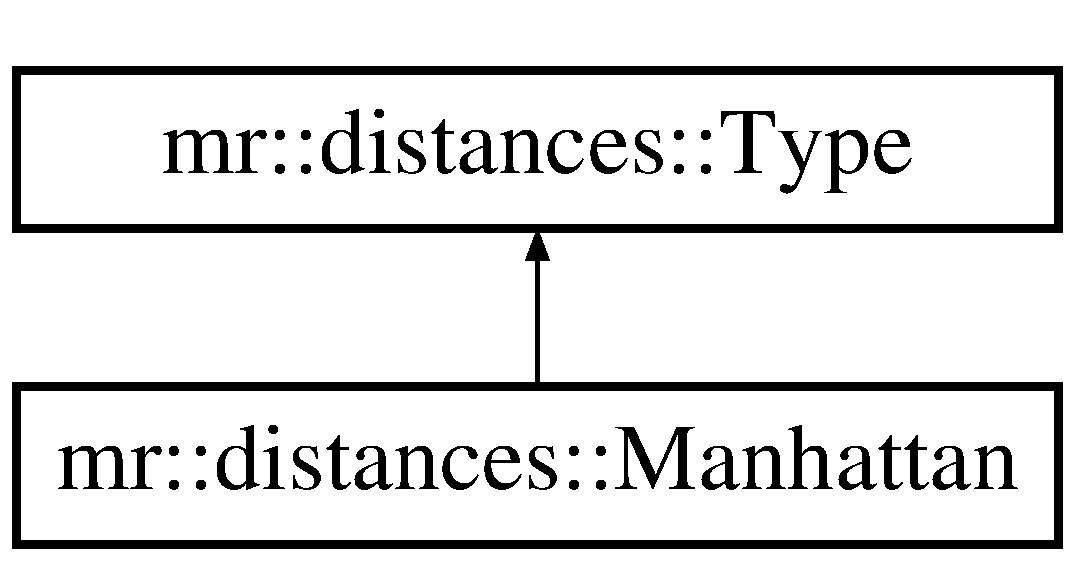
\includegraphics[height=2cm]{structmr_1_1distances_1_1Manhattan}
\end{center}
\end{figure}
\subsection*{Public Member Functions}
\begin{CompactItemize}
\item 
mi\-Scalar {\bf operator()} (const {\bf vector} \&d) const 
\item 
mi\-Scalar {\bf operator()} (const {\bf vector} \&d, const {\bf vector} \&s) const 
\end{CompactItemize}


\subsection{Detailed Description}
Functor to calculate manhattan distance. 



\subsection{Member Function Documentation}
\index{mr::distances::Manhattan@{mr::distances::Manhattan}!operator()@{operator()}}
\index{operator()@{operator()}!mr::distances::Manhattan@{mr::distances::Manhattan}}
\subsubsection{\setlength{\rightskip}{0pt plus 5cm}mi\-Scalar mr::distances::Manhattan::operator() (const {\bf vector} \& {\em d}, const {\bf vector} \& {\em s}) const\hspace{0.3cm}{\tt  [inline, virtual]}}\label{structmr_1_1distances_1_1Manhattan_a1}




Implements {\bf mr::distances::Type} {\rm (p.\,\pageref{structmr_1_1distances_1_1Type_a1})}.\index{mr::distances::Manhattan@{mr::distances::Manhattan}!operator()@{operator()}}
\index{operator()@{operator()}!mr::distances::Manhattan@{mr::distances::Manhattan}}
\subsubsection{\setlength{\rightskip}{0pt plus 5cm}mi\-Scalar mr::distances::Manhattan::operator() (const {\bf vector} \& {\em d}) const\hspace{0.3cm}{\tt  [inline, virtual]}}\label{structmr_1_1distances_1_1Manhattan_a0}




Implements {\bf mr::distances::Type} {\rm (p.\,\pageref{structmr_1_1distances_1_1Type_a0})}.

The documentation for this struct was generated from the following file:\begin{CompactItemize}
\item 
{\bf mr\-Distances.h}\end{CompactItemize}
